\section{Формула Грина.}
\subsection{Вывод формулы.}

\begin{minipage}{50mm}
\begin{figure}[H]
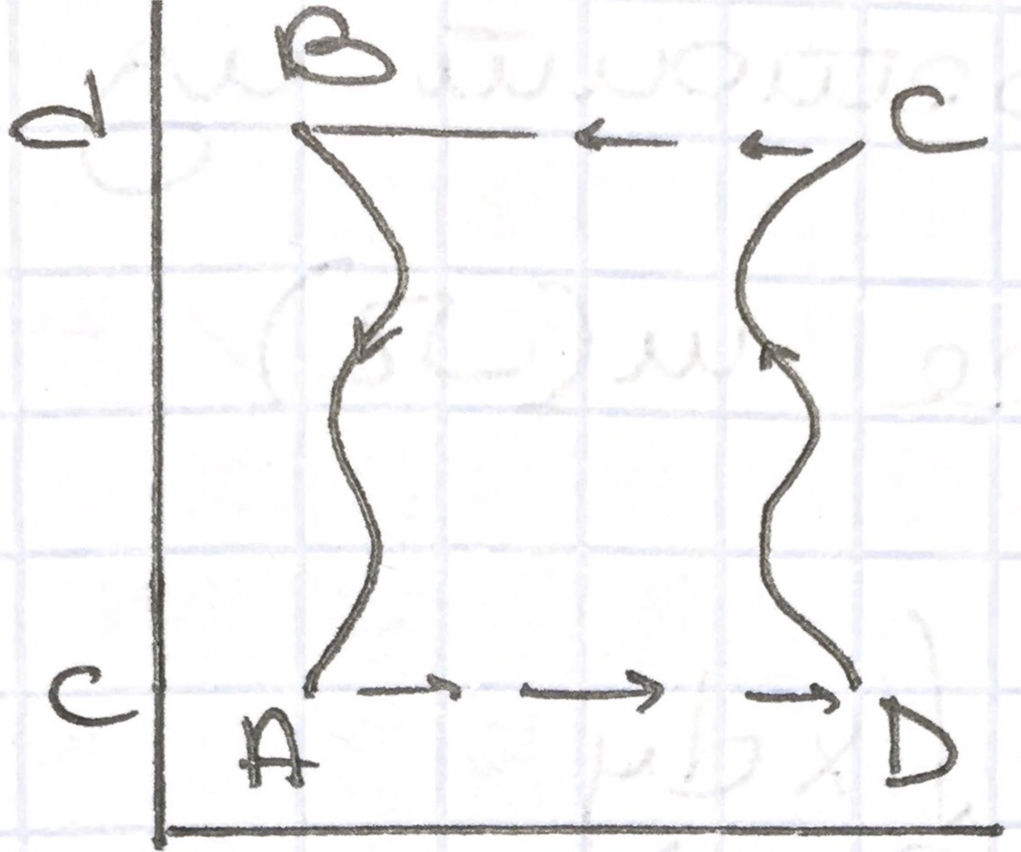
\includegraphics[width=50mm]{img1}
\end{figure}
\end{minipage}
~
\begin{minipage}{120mm}
\textbf{I случай.} $\Omega \subset \mathscr{E}$ элементарная область относительно $Oy$,\\
 $y=\varphi(x),\,y\hm{=}\psi(x),\,\psi(x)\leqslant\varphi(x)\,\forall x\in[a,b]$\\
$\omega=P(x,y),\,\omega=\frac{\partial P}{\partial y}(x,y)$ непрерывна в $\overline{\Omega}$\\
$\psi,\,\varphi$  --- непрерывны на $[a,b]$

$
\iint_\Omega \frac{\partial P}{\partial y}(x,y) dx dy = \int_{a}^{b}dx\int_{\psi}^{\varphi}\frac{\partial P}{\partial y}(x,y)dy=\int_{a}^{b}P(x,\varphi(x))dx\hm{-}\int_{a}^{b}P(x,\psi(x))dx=\int_{BC}P(x,y)dx-\int_{AB}P(x,y)dx=-\int_{CB}P(x,y)dx\hm{-}\int_{AD}P(x,y)dx=-\oint_{ADCBA}P(x,y)dx=-\oint_{d\Omega}P(x,y)dx$
\end{minipage}
$$\int_{BA} P(x,y)dx=\int_{DC}P(x,y)dx=0 \Rightarrow \iint_\Omega\frac{\partial P}{\partial y}(x,y)dxdy=-\oint_{d\Omega}P(x,y)dx$$
	

\begin{minipage}{120mm}
\textbf{II случай.} $\Omega \subset \mathscr{E}$ элементарная область относительно $Ox$, $x=\varphi(y),\,x=\psi(y),\,\psi(y)\leqslant\varphi(y)\forall y\in[c,d]$\\
$\omega=Q(x,y),\,\omega=\frac{\partial Q}{\partial x}(x,y)$ непрерывна в $\overline{\Omega}$\\
$\psi,\,\varphi$  --- непрерывны на $[c,d]$\\
$
\iint_\Omega \frac{\partial Q}{\partial x}(x,y) dx dy = \int_{c}^{d}dy\int_{\psi(y)}^{\varphi(y)}\frac{\partial Q}{\partial x}(x,y)dx=\int_{c}^{d}Q(\varphi(y),y)dy\hm{-}\int_{c}^{d}Q(\psi(y),y)dy=\int_{DC}Q(x,y)dy+\int_{BA}Q(x,y)dy\hm{=}\oint_{ADCBA}Q(x,y)dy=\oint_{d\Omega}Q(x,y)dy$
\end{minipage}
~
\begin{minipage}{50mm}
	\begin{figure}[H]
		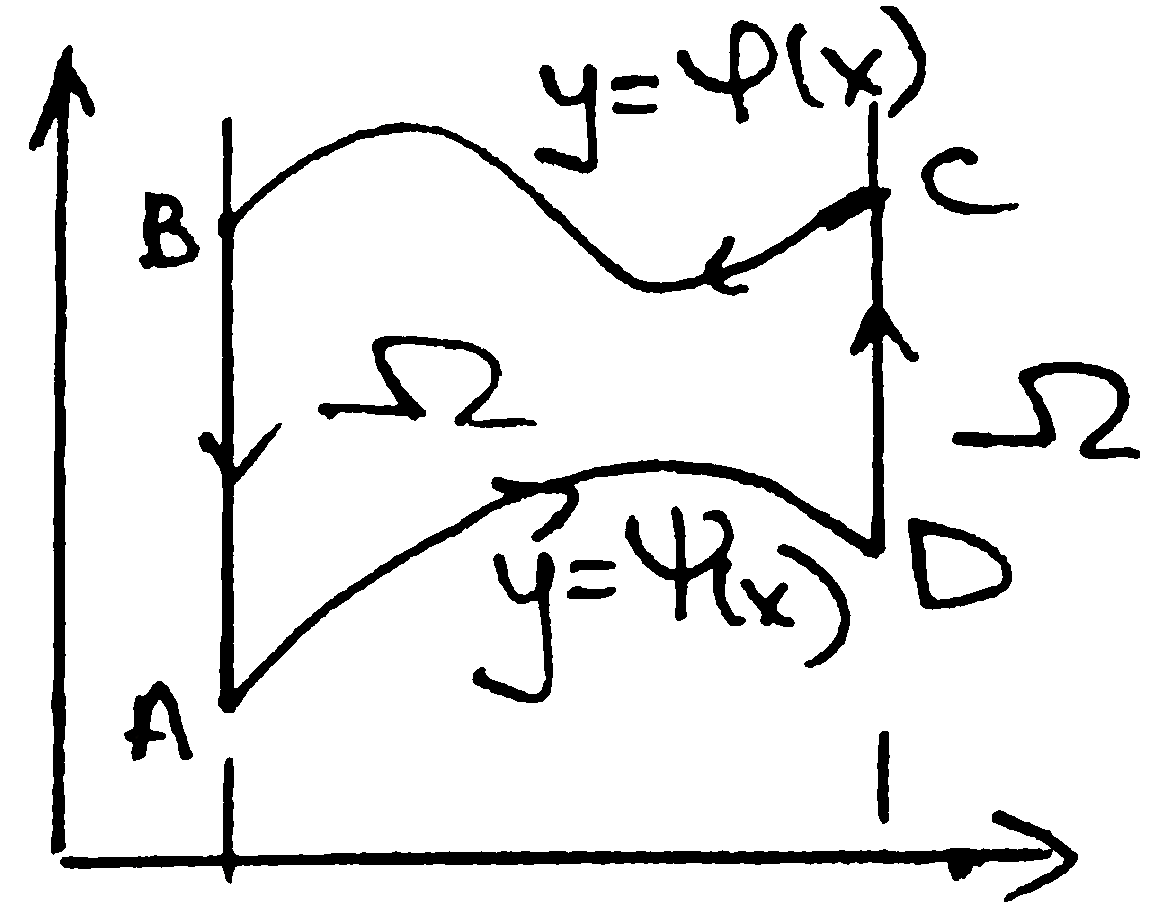
\includegraphics[width=50mm]{img2}
	\end{figure}
\end{minipage}

Выше мы воспользовались тем, что $\int_{AD}Q(x,y)dy=\int_{CB}Q(x,y)dy=0$ 

\begin{theorem}\label{th:1} Пусть область $\Omega$ представляет собой объединение конечного числа измеримых областей элементарных относительно $Oy$. $\overline{\Omega}=$\tmb{k}{\cup}{j=1}$\overline{\Omega'_i},\,\overline{\Omega''_i},\;i=\overline{1,k},\;j=\overline{1,k}$.\\
Функции $P,Q,\frac{\partial P}{\partial y}, \frac{\partial Q}{\partial x}$ непрерывны в $\overline{\Omega}$, тогда справедлива формула Грина:
$$ \iint_\Omega\left[\frac{\partial Q}{\partial x}(x,y)-\frac{\partial P}{\partial y}(x,y)\right]dxdy=\int_{\partial\Omega}P(x,y)dx+Q(x,y)dy $$
\end{theorem} 
\begin{theorem_nu}[\textbf{1'}]\label{th:1'} Если граница $\partial \Omega$ ограниченной области $\Omega\subset \mathscr{E}^2$ состоит из конечного числа кусочно гладких контуров и эти функции непрерывны, то имеет место формула Грина:
$$ \iint_\Omega\left[\frac{\partial Q}{\partial x}(x,y)-\frac{\partial P}{\partial y}(x,y)\right]dxdy=\int_{\partial\Omega}P(x,y)dx+Q(x,y)dy $$
\end{theorem_nu}  
\section{Некоторые приложения формулы Грина.} 
\subsection*{A. Вычисление плоских измеримых областей.} 
\begin{sentence} Если граница $\partial \Omega$ ограниченной области $\Omega\subset \mathscr{E}^2$ состоит из конечного числа кусочно гладких контуров, то ее $m(\Omega)$ определяется из формулы:
\end{sentence}
\begin{equation*}
m(\Omega)=1/2\int_{\partial\Omega}\left[xdy-ydx\right]
\end{equation*} 
\begin{proof} По формуле Грина $\int_{\partial\Omega}\left[xdy-ydx\right]=2\iint_\Omega dxdy=2m(\Omega)$
\end{proof}
\subsection*{B. Условия, при которых дифференциальное выражение(дифф. форма) $Pdx+Qdy$ является дифференциалом некоторой функции $f= \\=f(x,y)$} 
\begin{theorem}\label{th:2}Пусть область $\Omega\subset\mathscr{E}^2$ --- произвольная область и функции $P$ и $Q$ непрерывны на $\overline{\Omega}$, тогда следующие условия эквивалентны:
\begin{enumerate}
	\item $\oint_\varGamma P(x,y)dx+Q(x,y)dy$, где $\varGamma$ --- произвольная замкнутая кусочно гладкая кривая, причем $\varGamma\subset\Omega$
	\item $z'=(x',y'),\, z'' = (x'' , y'')$ --- т. области $\Omega,\;\varGamma\subset\Omega$ -- кусочно гладкая кривая, соединяющая точки $z'$ и $z''$, то $\int_\varGamma Pdx+Qdy$ не зависит от кривой $\varGamma$, а только от т. $z'$ и $z''$.
	\item Существует функция $w=f(x,y)$ такая, что $df=Pdx+Qdy$, при этом если $z',\,z''\in \Omega$ и $\varGamma\subset \Omega$ --- кусочно гладкая кривая, соединяющая точки $z'$ и $z''$, то \begin{equation}
	\int_\varGamma Pdx+Qdy=f(z'')-f(z')
	\label{eq:star}
		\end{equation}
\end{enumerate}
\end{theorem}
\begin{proof}
$\text{Схема доказательства: }1\Rightarrow2\Rightarrow3\Rightarrow1$
\paragraph{\fbox{$1\Rightarrow2$}}  $z',\,z''\in \Omega,\,\varGamma',\,\varGamma''$ --- кусочно гладкие кривые соединяющие точки $z'$ и $z''$\\
$\varGamma=\varGamma'\cup(\varGamma'')^-	$ --- замкнутуая кусочно гладкая кривая 
\\
$0\overset{1}{=}\int_\varGamma Pdx+Qdy= \int_{\varGamma'} Pdx+Qdy -\int_{\varGamma''} Pdx+Qdy\Rightarrow\int_{\varGamma'} Pdx+Qdy=\int_{\varGamma''} Pdx+Qdy$
\paragraph{\fbox{$2\Rightarrow3$}} $z^0=(x_0,y_0)\in\Omega;\; \varGamma_z\subset\Omega$ --- кусочно гладкая кривая, соединяющая т. $z_0$ и $z=(x,y)$\\
$$f(z)=f(x,y)=\int_{\varGamma_z}Pdx+Qdy.$$
$z=(x,y),\,z'=(x+\Delta x ,y),\,z' \in\Omega$ и $[z,\,z']\subset\Omega$ 
\begin{multline*}
\Delta f(z, \Delta x)=f(x+\Delta x,y)-f(x,y)=\int_{\varGamma\{z,z'\}}Pdx+Qdy=\int_{x}^{x+\Delta x}P(t,y)dt=\\=P(x+\theta\Delta x,y)\Delta x, 0<\theta<1\end{multline*}
$\dfrac{f(x+\Delta x,y)-f(x,y)}{\Delta x}=P(x+\theta\Delta x,y)\Rightarrow\pdd{f}{x}(x,y)=P(x,y)$ аналогично $\pdd{f}{y}(x,y)=Q(x,y)$\\
$\varGamma = \{(x,y), x=\varphi(t), y=\psi(t),\, \alpha\leqslant t\leqslant \beta\},\;z'=(\varphi(\alpha),\psi(\alpha)),\;z''=(\varphi(\beta),\psi(\beta))$\\
$\int_\varGamma Pdx+Qdy=\int_{\alpha}^{\beta}[P(\varphi(t),\psi(t))\cdot\varphi'(t)+Q(\varphi(t),\psi(t))\cdot\psi'(t)]dt=\int_{\alpha}^{\beta}\left[\pdd{f}{x}x'+\pdd{f}{y}y'\right]dt\hm{=}\\=\int_{\alpha}^{\beta}\frac{d}{dt}[f(\phi(t),\psi(t))]dt=f(\varphi(\beta),\psi(\beta))-f(\varphi(\alpha),\psi(\alpha))=f(z'')-f(z')$
\paragraph{\fbox{$3\Rightarrow1$}} $\varGamma\subset\Omega$ --- кусочно гладкая замкнутая кривая, т.е. $z'$ и $z''\Rightarrow \eqref{eq:star} \Rightarrow \int_\varGamma Pdx+Qdy=0$\\
\end{proof}
\begin{theorem}\label{th:3} Если в условии теоремы \ref{th:2} $\Omega\subset\mathscr{E}^2$ --- односвязная область и функция $P,Q,\frac{\partial P}{\partial y},\frac{\partial Q}{\partial x}$ непрерывны в $\overline{\Omega}$, то по условиям 1--3 теорема 2 эквивалентна следующему условию:\\
4. $\frac{\partial P}{\partial y}(x,y)=\frac{\partial Q}{\partial x}(x,y)\;\forall(x,y)\subset\Omega$
\end{theorem}
\begin{proof}
\fbox{$3\Rightarrow4$} $\quad\frac{\partial P}{\partial y}=\frac{\partial}{\partial y}\left(\frac{\partial f}{\partial x}\right)=\frac{\partial}{\partial x}\left(\frac{\partial f}{\partial y}\right)=\frac{\partial Q}{\partial x}$\\
\fbox{$4\Rightarrow1$}$\quad \varGamma\subset\Omega$ простая кусочно гладкая замкнутая кривая $\varGamma=\partial \Omega^*,\,\Omega^*\subset\Omega$.\\
$\int_{\varGamma}Pdx+Qdy=\iint_{\Omega^*}\left[\frac{\partial Q}{\partial y}-\frac{\partial P}{\partial x}\right]dxdy=0$
\end{proof} 
Легко доказать, если $\varGamma$ имеет конечное число точек самопересечения. Для произвольной кусочно гладкой замкнутой кривой все остальное справедливо.